From Replica Exchange Molecular Dynamics\cite{Sugita1999}, the hamiltonian representing the potential energy of the system can be written as sum of respective contributions, separated into protein-protein, protein-water and water-water:
\begin{center}
    \begin{equation}
        E_{n}^{REMD}(X_{n}) = \lambda_{n}^{pp} E_{pp}(X_{n}) + \lambda_{n}^{pw} E_{pw}(X_{n}) + \lambda_{n}^{ww} E_{ww} (X_{n})
    \label{eq:remd_hamiltonian}
    \end{equation}
\end{center}

$\lambda_{n}^M$ is the scaling factor, where $M=\{ pp, pw, ww\}
$ which scales the corresponding energy term. For REST2\cite{Wang2011}, $\lambda_n^{ww}=1$, $\lambda_n^{pp}=(\lambda_n^{pw})^2=\lambda_n$, for simplicity the REST2 hamiltonian simplifies to:
% import simplified hamiltonian of REST2
\begin{center}
    \begin{equation}
        E_{n}^{REST2}(X_{n}) = \lambda_{n} E_{pp}(X_{n}) + \sqrt{\lambda_{n}} E_{pw}(X_{n}) +  E_{ww} (X_{n})
        \label{eq:rest2_hamiltonian}
    \end{equation}
\end{center}
% import lambda scaling equation
where,
\begin{center}
    \begin{equation}
        % \lambda_{n}^{pp}=\frac{\beta_{n}}{\beta_{0}} \ ; \quad \lambda_{n}^{pw}=\sqrt{\frac{\beta_{n}}{\beta_{0}}} \ ; \quad \lambda_{n}^{ww}=1;   
        \lambda_n = \frac{\beta_{n}}{\beta_{0}}
    \label{eq:lambda_scaling}     
    \end{equation}
\end{center}
% import temperature factor expression
and $\beta_{n}=\frac{1}{k_{B}T_{n}}\ for\ n=\{0,1,2,\ldots,n_{replica}\}$. 

Upon implementation of metropolis acceptance criteria with detail balance being satisfied, the acceptance probability between state $n$ and $n+1$ is given by:
\begin{center}
    \begin{equation}
        \Delta_{n,n+1} = (\beta_{n} - \beta_{n+1}) \Big[(E_{pp}(X_{n+1}) - E_{pp}(X_{n})) + \frac{\sqrt{\beta_{0}}} {\sqrt{\beta_{n}}+\sqrt{\beta_{n+1}}} (E_{pw}(X_{n+1}) - E_{pw}(X_{n}))\Big].
        \label{eq:rest2_AR}
    \end{equation}
\end{center}

By excluding the solvent-solvent interactions w.r.t. scaling, the contribution to the acceptance criteria contains less degrees of freedom relative to REMD resulting in better acceptance between replicas.

Upon investigation, disordered proteins containing hydrophobic residues undergo conformational collapse with respect to scaling  $E^{pw}$ to higher effective temperatures. 
This outcome is unfavorable when attempting to capture a representative ensemble as hydrophobic collapse reduces the overall sampling of the proteins conformational ensemble. % We need to say something here to the effect: REST2's ability to enhance hydrophobic interactions is synonamous with reducing the quality of the solvent, water. 
\citeauthor{Zhang2023} \citeyear{Zhang2023} provided a basis for biasing the scaling such that protein collapse is minimized or negated, with the hamiltonian:
\begin{center}
    \begin{equation}
        E_{n}^{REST3}(X_{n}) = \lambda_{n} E_{pp}(X_{n}) + \kappa_n\sqrt{\lambda_{n}} E_{pw}(X_{n}) +  E_{ww} (X_{n}).
        \label{eq:rest2_hamiltonian}
    \end{equation}
\end{center}

%add in info about variables, what are they?
By incorporating the scaling factor $\kappa_n$, where $n=\{1,2,3,\ldots,n_{replica}\}$, the dampening effect of $\lambda$ is deminished. 
To accomplish this $\kappa_n$ exist in the range $[1.0,1.06]$. 
Due to the method of implementation the base replica (unscaled topology), following conversion of the topologies to REST3 \cite{Zhang2023} formalism using combination rule 1 instead of 2, does not match the potential energy of the original topology. 
The implementation of REST3 by \citeauthor{Zhang2023} target scaling of protein-water lj parameters by means of computing C6 and C12 parameters. 
There exists a descrepancy between the unscaled-converted topology and the original topology via machine error of switching the potential from combination rule 2 to combination rule 1 in GROMACS, however, the conformational sampling desired is observed. When $\lambda$ scaling is applied, as in REST2, the well depth of the LJ potential is deminished, Figure 
\begin{figure}
    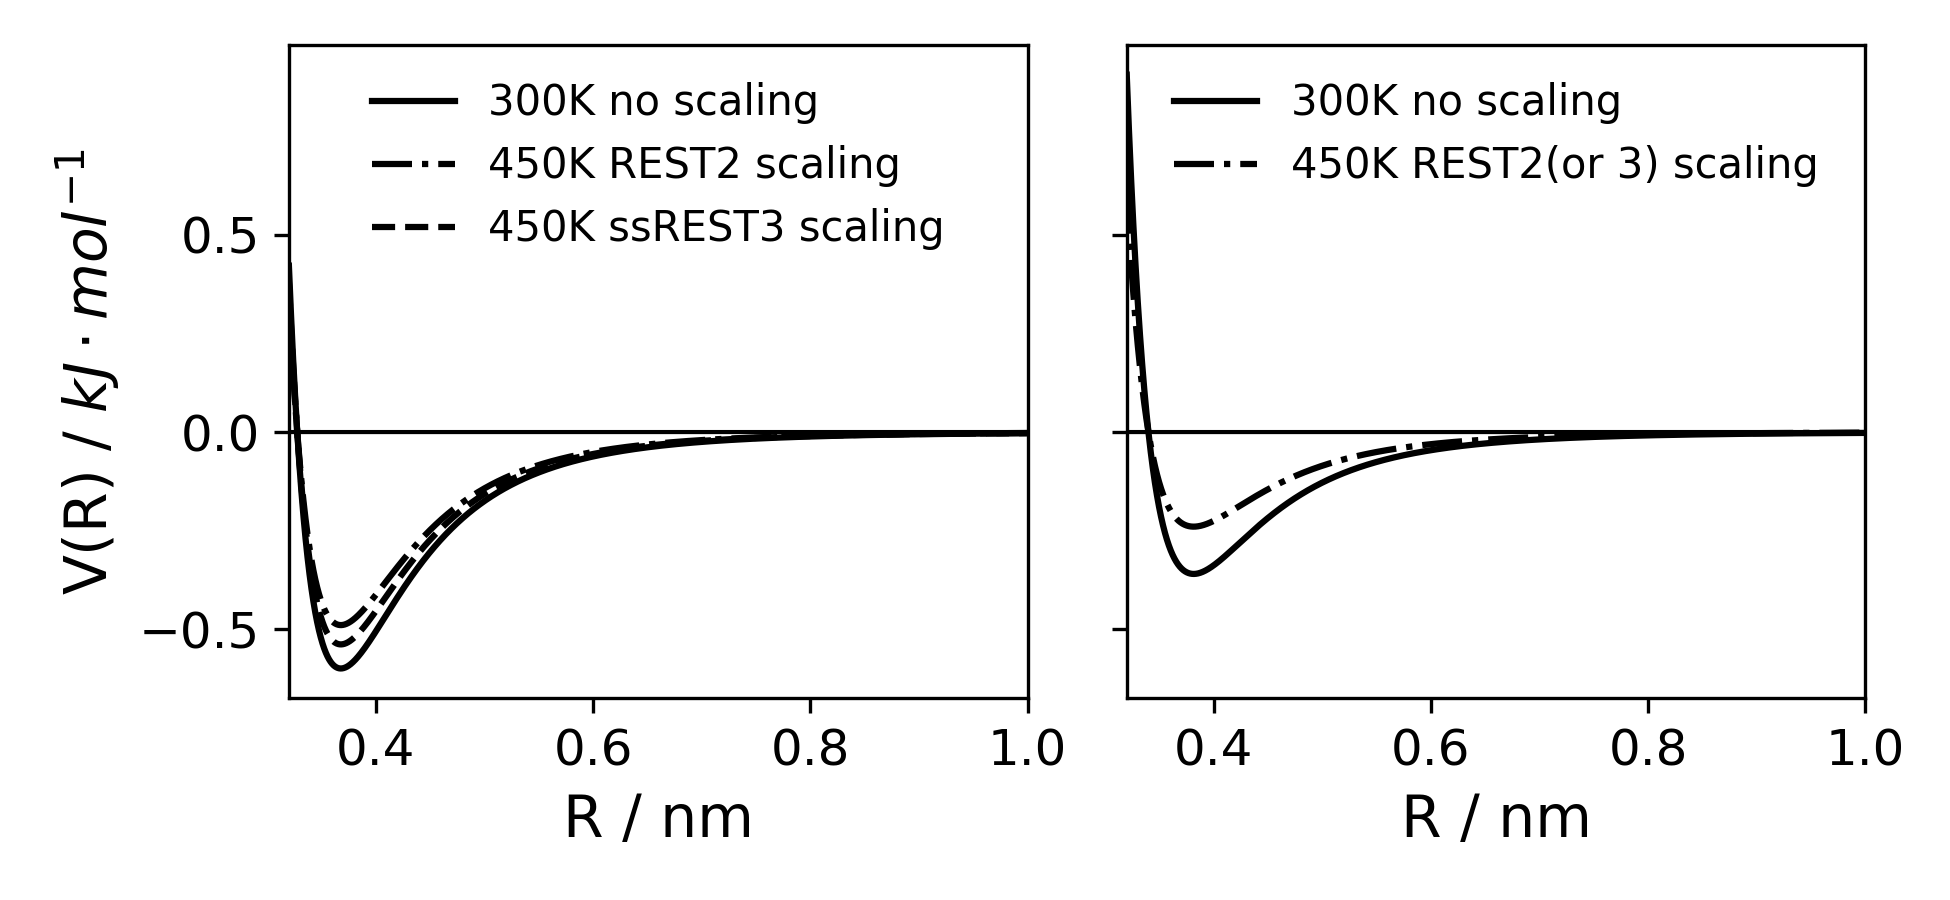
\includegraphics[width=\textwidth]{../Figure_a/fig_a.png}
    \caption{LJ potential for differing values of epsilon for the same atom-atom pair.}
    \label{fig:lj_curves}
\end{figure}
where $\lambda_n$ is still applied to the protein in the same fashion as REST2 \cite{Wang2011} and solvent scaling is applied to the water oxygen via the well-depth, $\epsilon_{OW}$, borrowing from the methods described in \citeauthor{Best2010} \citeyear{Best2010}. 
To overcome the inherent mechanics within GROMACS\cite{VanDerSpoel2005}, nonbonded overrides are implemented for water-water and water-ion.
Additionally, one can override water-cosolute if scaling is not desired between the two. 
For ssREST3, $\kappa_n$ is defined by the expression, 
\begin{center}
    \begin{equation}
        \kappa_{n}=\kappa_{low}*\exp{ \biggl(n*\frac{\log(\kappa_{high}/\kappa_{low})}{N_{r}-1}\biggr)} \ ; \quad 1.00 \leq \kappa_{n} \leq 1.10.
    \label{eq:kappa_scaling}
    \end{equation}
\end{center}

To understand where $\kappa_n$ is applied, we start with an expression for the Lennard-Jones potential between the $i^{th}$ protein atom and the water oxygen,
\begin{center}
    \begin{equation}
        \sqrt{\lambda_n}\cdot\kappa_n\cdot E_{i,OW}^{lj} = \sqrt{\lambda_n}\cdot \kappa_n \cdot 4 \cdot\epsilon_{i,OW}\Big[ \Big( \frac{\sigma_{i,OW}}{r}\big)^6 -  \Big( \frac{\sigma_{i,OW}}{r}\big)^{12} \Big]
    \label{eq:lj_potential}
    \end{equation}
\end{center}

The CHARMM and Amber forcefields both conform to the Lorentz-Berthelot rules, i.e. $\epsilon_{i,j}=\sqrt{\epsilon_i\cdot \epsilon_j}$. From Equation \ref{eq:lj_potential} we can refactor $\sqrt{\lambda_n}\cdot\kappa_n\cdot\epsilon_{i,OW}$ to clarify which forcefield parameters are scaled. 
\begin{center}
    \begin{equation}
        \epsilon_{p:OW}=(\epsilon_{p:p}^{rescaled} * \epsilon_{OW:OW}^{rescaled})^{\frac{1}{2}}=\lambda_{n}^{pw}\kappa_{n}*(\epsilon_{p:p} * \epsilon_{OW:OW})^{\frac{1}{2}}
    \label{eq:wat_scaling}
    \end{equation}
\end{center}

The sections that follow are the Materials, Methods and Notes sections.
Within the materials sections we detail the required software and minimum hardware requirements to perform REST based simulations.
The Methods sections contains a complete description with examples on how to create and produce REST2 and ssREST3 simulations following an example simulation involving $\alpha$-synuclein and a small molecule. Additionally, we include a few examples of analysis to test for convergence. Lastly, we provide various Notes in the last section. 